\documentclass[10pt,a4paper]{article}
\usepackage[left=20mm,right=20mm,top=15mm,bottom=15mm]{geometry}
\usepackage{amsmath,booktabs,graphicx}
\usepackage{fontspec,xeCJK}
\IfFontExistsTF{Songti TC}{\setCJKmainfont{Songti TC}}{\setCJKmainfont{Noto Serif CJK TC}}
\usepackage[hidelinks]{hyperref}
\setlength{\parindent}{0pt}
\setlength{\parskip}{3pt}
\title{Robust Multi-Objective Bayesian Optimization\\
for Signal Timing at Taipei's Gongguan Intersection}
\author{林采穎 (Lin Tsai-Ying) \quad b13705007}
\date{}
\begin{document}
\maketitle
\vspace{-12mm}

\section{Problem and motivation}

Taipei reopened the former Gongguan Roundabout as a conventional intersection on September 29, 2025 \cite{taipei}. When I ride through Gongguan, my bus sometimes waits through several signal cycles. On foot, the wait has felt acceptable. Can peak-period timing reduce bus delay while keeping pedestrian and general-traffic delays acceptable, even when demand shifts?

Traffic engineers typically start from an existing plan, adjust green splits using traffic counts and queue observations, and check the changes in simulation or on site. Google's Project Green Light uses Google Maps driving trends to recommend adjustments for engineers to review \cite{greenlight}. A timing change that helps on a typical day can worsen queues during a surge. BO complements manual tuning by using all three measured objectives and their uncertainty to prioritize the next trial. A grid with 10 settings per variable requires 100 plans. The prototype evaluates 20, an 80\% smaller budget, with no assumption that the searches find equivalent solutions.

\section{Design variables, objectives, and evaluation cost}

A timing plan is $x=(C,r)$, where the cycle length $C$ ranges from 100 to
160 seconds and the main-axis share $r$ ranges from 0.45 to 0.65. Each of
the two phases reserves 25 seconds of green and 5 seconds of clearance.
The remaining $C-60$ seconds are split between the main and cross axes
according to $r$. Pedestrians crossing the main axis may start during
the cross-axis green, except during its final 12 seconds, which are
reserved for clearance. These values define the synthetic design space. For example, $C=130$ s and
$r=55\%$ give the main and cross axes 63.5 s and 56.5 s of green.

For a demand scenario $s$, the simulator estimates three quantities,
all in seconds and all to be minimized:
\[
f(x,s) = \bigl(\text{mean bus queueing delay},\;
                 \text{pedestrian P95 wait},\; \text{mean general-traffic delay}\bigr).
\]
The prototype uses FIFO vehicle queues and simulates one hour of random arrivals under typical peak demand, clustered bus arrivals, and cross-axis peak demand. The two variables keep the demonstration small. Field deployment could also tune individual phase lengths and offsets between neighboring signals.

Each candidate needs $3\times4=12$ simulation runs. The 20-plan search requires 240 runs, compared with 1,200 for the example grid under identical replication. At an illustrative 2 minutes per calibrated run, a single candidate would take 24 minutes of serial simulation. Field validation spans multiple comparable peak periods. The prototype substitutes fast synthetic simulation for these more costly evaluations.

\section{Bayesian optimization workflow}

Engineers set the scenarios and budget. The system tests four Sobol plans, then uses three Gaussian-process (GP) models and BoTorch's qLogNEHVI \cite{botorch} to choose candidates with promising expected Pareto hypervolume gains. Simulated delays vary with arrivals. Each scenario metric averages four shared random samples to reduce noise and enable fairer comparisons. The system updates the GPs with each plan's scores.

The prototype stops at 20 plans. In practice, engineers could also stop after hypervolume gains stay below a threshold. On the Pareto front they could screen for pedestrian P95 $\leq70$ s, then choose the lowest bus delay among plans meeting that illustrative limit. The benchmark instead uses a fixed equal-weight sum of the three training scores scaled by 150 s and tests the selected plan on held-out demand.

\begin{center}
\setlength{\unitlength}{1pt}
\begin{picture}(430,58)
\put(0,27){\framebox(97,28){\footnotesize\shortstack{Set scenarios\\and budget}}}
\put(111,27){\framebox(97,28){\footnotesize\shortstack{Propose a plan\\Sobol or qLogNEHVI}}}
\put(222,27){\framebox(97,28){\footnotesize\shortstack{Simulate and score\\all three objectives}}}
\put(333,27){\framebox(97,28){\footnotesize\shortstack{Record results and\\update three GPs}}}
\put(97,41){\vector(1,0){14}}
\put(208,41){\vector(1,0){14}}
\put(319,41){\vector(1,0){14}}
\put(382,27){\line(0,-1){11}}
\put(382,16){\line(-1,0){222}}
\put(160,16){\vector(0,1){11}}
\put(160,3){\makebox(222,10){\scriptsize Fewer than 20 plans}}
\end{picture}

\small At 20 plans, show the Pareto front, choose a representative plan, and test it on held-out demand.
\end{center}

\newpage
\section{Why optimize across demand scenarios?}

More main-axis green can help buses while increasing waits for pedestrians or cross-axis traffic. MOBO shows those trade-offs before engineers choose priorities. The objectives are measured directly, so pairwise preference feedback adds little here. Transfer BO could warm-start future searches at related intersections.

A bus platoon can leave a queue across cycles. To keep quieter scenarios from masking such delays, the prototype uses a finite-scenario maximum, $g_j(x)=\max_s f_j(x,s)$, for each objective. Kinnunen et al. \cite{kinnunen} motivate this focus on demand uncertainty with a distinct robust satisficing method that seeks to meet a threshold across a wider range of conditions.

\section{Prototype results and limitations}

Each search method was run four times with shared initial plans and
equal evaluation budgets. The benchmark included uniform random search
after initialization and a fixed synthetic plan of 130 seconds and a
55\% main-axis share. Each selected plan was tested on higher arrival
rates and 12 new random arrival samples per scenario. Random search and worst-scenario MOBO
use the same rule to select a representative plan.

\begin{center}
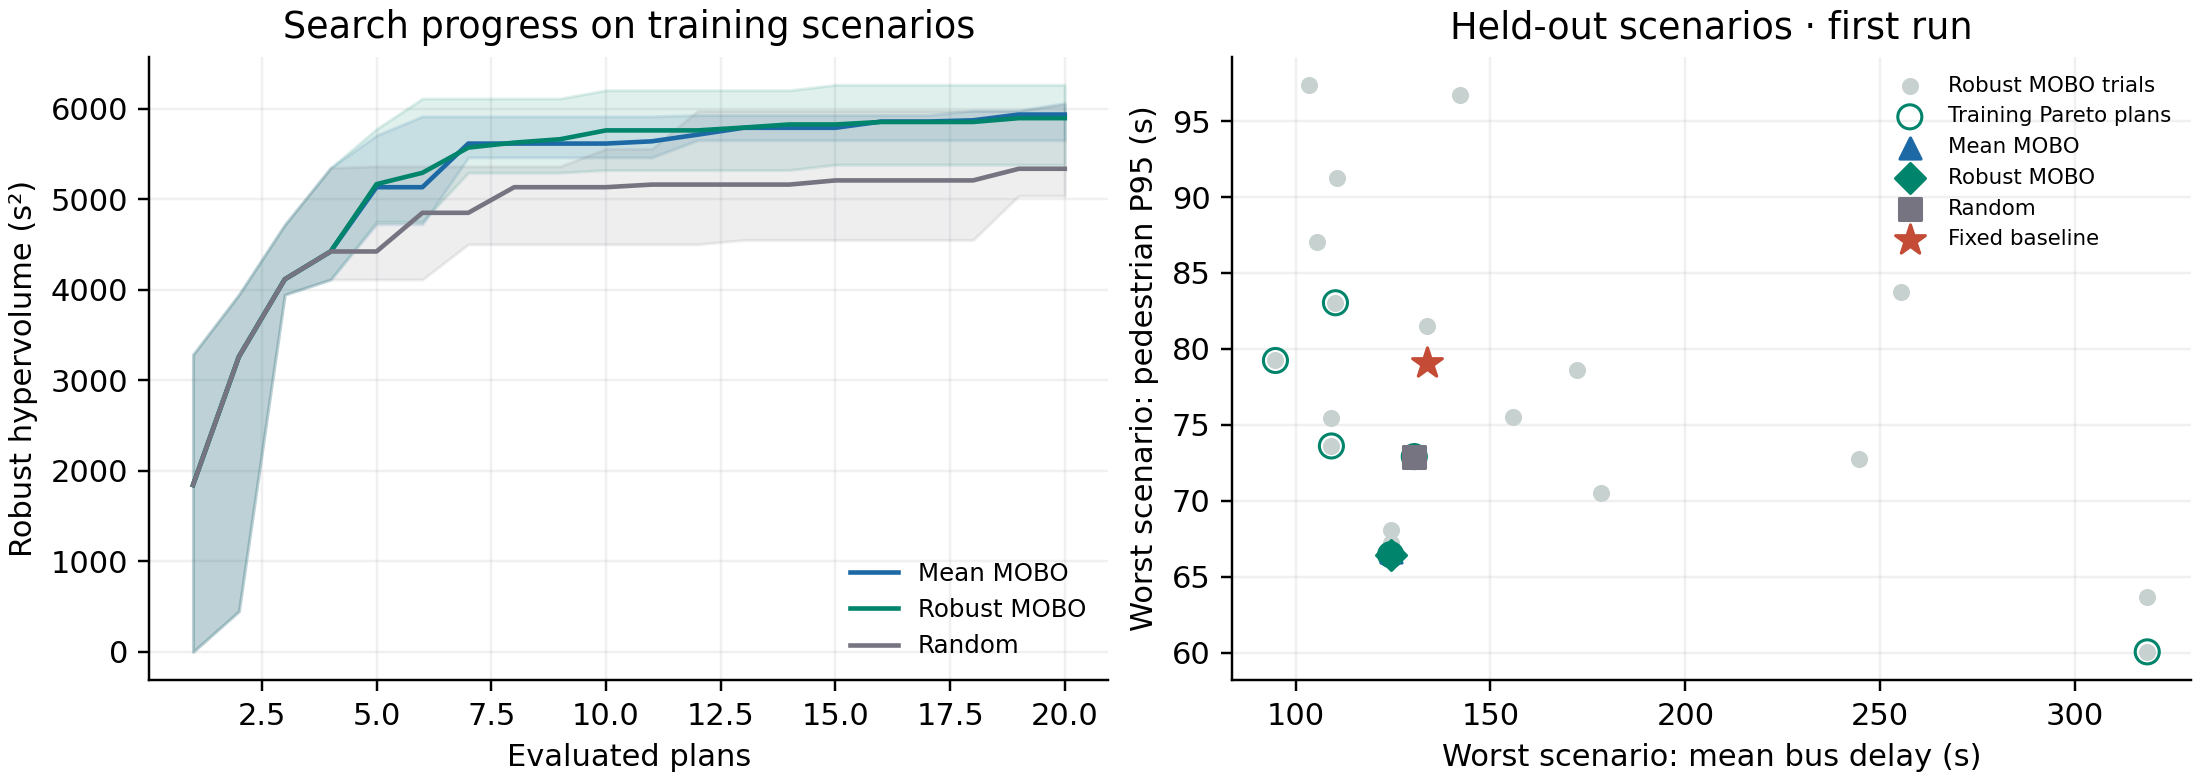
\includegraphics[width=.92\linewidth]{../results/results.png}

\small Figure 1. Training hypervolume (left, higher is better) and
held-out scores for the first run (right). Candidate dot colors show general-traffic delay.
Hollow markers identify plans on the training Pareto front.
\end{center}

\begin{center}
\begin{tabular}{lrrr}
\toprule
Method & Bus mean (s) & Walk P95 (s) & General traffic mean (s) \\
\midrule
Fixed synthetic plan & 133.7 & 79.1 & 38.5 \\
Average-scenario MOBO & 124.4 & 66.6 & 48.7 \\
Worst-scenario MOBO & 124.4 & 66.8 & 48.8 \\
Random search & 102.3 & 73.4 & 57.3 \\
\bottomrule
\end{tabular}

\small Table 1. Median across four runs of each metric's worst
held-out scenario. Lower values are better.
\end{center}

Random search had the lowest median bus delay. Both MOBO methods had lower pedestrian and general-traffic delays than random search, and worst-scenario MOBO had about 12\% higher median training hypervolume. The fixed plan had the lowest general-traffic delay.

The two MOBO methods had similar holdout results. Across 182 distinct timing plans pooled from all searches in \texttt{trials.csv}, mean and worst-scenario rankings for each training objective had Spearman $\rho$ of 0.99 (bus), 1.00 (pedestrian, rounded), and 0.92 (general traffic). This agreement may explain the similar results. More extreme demand could separate the rankings, a hypothesis for future testing. Field use requires measured demand, actual phase timings, and checks for spillback and pedestrian clearance.

\begin{thebibliography}{9}\small
\bibitem{taipei} Taipei City New Construction Office.
\href{https://english.nco.gov.taipei/News_Content.aspx?n=C43859DE9907C884\&s=B408C94159CBDBA6}{Gongguan Roundabout improvement project}.
\bibitem{greenlight} Google Research.
\href{https://sites.research.google/gr/greenlight/}{Project Green Light}.
\bibitem{botorch} BoTorch.
\href{https://botorch.org/docs/v0.16.1/tutorials/multi_objective_bo}{Multi-objective Bayesian optimization tutorial}.
\bibitem{kinnunen} Kinnunen, S., Mikkola, P., Niskanen, A., and Klami, A.
\href{https://proceedings.mlr.press/v337/kinnunen26a.html}{Maximally Robust Satisficing Bayesian Optimization}. UAI, 2026.
\end{thebibliography}

\end{document}
